\documentclass[aspectratio=169, 10pt]{beamer}

% Theme & Styling
\usetheme{Madrid}
\usecolortheme{seahorse}
\setbeamertemplate{footline}[frame number]

\definecolor{primaryblue}{RGB}{15, 32, 39}
\definecolor{accentteal}{RGB}{49, 151, 149}
\definecolor{darkteal}{RGB}{32, 58, 67}
\definecolor{cardbg}{RGB}{245, 247, 250}

\setbeamercolor{palette primary}{bg=primaryblue,fg=white}
\setbeamercolor{palette secondary}{bg=darkteal,fg=white}
\setbeamercolor{palette tertiary}{bg=accentteal,fg=white}
\setbeamercolor{titlelike}{parent=palette primary}
\setbeamercolor{structure}{fg=accentteal}

\usepackage{amsmath, amssymb, amsfonts}
\usepackage{booktabs}
\usepackage{graphicx}
\usepackage{tikz}
\usetikzlibrary{shapes.geometric, arrows.meta, positioning}

\usepackage{listings}
\usepackage[scaled=0.88]{inconsolata}

\definecolor{codegreen}{rgb}{0,0.55,0}
\definecolor{codegray}{rgb}{0.45,0.45,0.45}
\definecolor{codepurple}{rgb}{0.58,0,0.82}
\definecolor{codeblue}{RGB}{0, 102, 204}
\definecolor{codekw}{RGB}{170, 13, 145}
\definecolor{backcolour}{rgb}{0.96,0.96,0.96}

\lstdefinestyle{pystyle}{
    language=Python,
    backgroundcolor=\color{backcolour},   
    commentstyle=\color{codegreen}\itshape,
    keywordstyle=\color{codekw}\bfseries,
    morekeywords={self, super, as, with, True, False, None, return, yield, import, from, def, class, if, else, elif, for, in, while, break, continue, try, except, lambda},
    keywordstyle=[2]\color{codeblue}\bfseries,
    morekeywords=[2]{nn, Module, LSTM, Sequential, Linear, LayerNorm, ReLU, Dropout, torch, sigmoid, GradientBoostingRegressor, LpProblem, LpVariable, LpMaximize, lpSum, fit, predict, squeeze, forward, zeros, where, clip, maximum, mean, std, array, pulp, np},
    numberstyle=\tiny\color{codegray},
    stringstyle=\color{codepurple},
    basicstyle=\ttfamily\scriptsize,
    columns=flexible,
    breakatwhitespace=true,         
    breaklines=true,                 
    keepspaces=true,                 
    numbers=left,                    
    numbersep=5pt,                  
    showspaces=false,                
    showstringspaces=false,
    showtabs=false,                  
    tabsize=2,
    xleftmargin=8pt,
    xrightmargin=8pt
}
\lstset{style=pystyle}

% Add section slide support
\AtBeginSection[]{
  \begin{frame}
  \vfill
  \centering
  \begin{beamercolorbox}[sep=8pt,center,shadow=true,rounded=true]{title}
    \usebeamerfont{title}\insertsectionhead\par%
  \end{beamercolorbox}
  \vfill
  \end{frame}
}

\title[CP-SSX Engine]{CP-SSX: Managerial Student Success Engine}
\subtitle{Mechanistic Explanations, Causal Uplift Analytics, and Constrained Resource Optimization}

\author[Group 4, MMLP]{
  \textbf{Group 4 -- Managerial Machine Learning in Python}\\[0.3em]
  \footnotesize
  Aayush Garg (PGPGC202500004) \quad Aditya Patwa (PGPGC202500008)\\
  Aniruddha Sharma (PGPGC202500105) \quad Arnav Dixit (PGPGC202500112)\\
  Saakshi Chowdhary (PGPGC202500260) \quad Yash Shukla (PGPGC202500183)
}
\institute[Group 4, MMLP]{Indian Institute of Management Ahmedabad}
\date{\today}

\begin{document}

\begin{frame}
  \titlepage
\end{frame}

\begin{frame}{Table of Contents}
  \tableofcontents
\end{frame}

% =============================================================================
\section{1. Data Description}
% =============================================================================

\begin{frame}{Real-World Student Foundation (4,424 Profiles)}
  \begin{itemize}
    \item \textbf{Dataset Foundation:} Built 100\% on actual published student records from the \textbf{UCI Machine Learning Repository} (Dataset ID 697: \textit{Predict Students' Dropout and Academic Success}).
    \item \textbf{Dynamic Temporal Signals (12 Weeks):}
      \begin{itemize}
        \item \textbf{Weekly Engagement Velocity:} Measures VLE page view acceleration and decay over time.
        \item \textbf{Procrastination Lag:} Average submission delays past assignment deadlines.
        \item \textbf{Academic Preparedness Index:} Composite score of prior qualifications and 1st-semester grades.
      \end{itemize}
    \item \textbf{Demographic \& Economic Factors:} Age, attendance mode, debt status, scholarship status, and unemployment rates.
  \end{itemize}
\end{frame}

\begin{frame}{Data Fields and Prediction Labels (UCI 697)}
  \begin{columns}[T]
    \begin{column}{0.48\textwidth}
      \begin{block}{Input Features (Covariates)}
        \begin{itemize}
          \item \textbf{Demographics:} Age, Gender, Nationality.
          \item \textbf{Socioeconomic:} Marital status, Debtor status, Tuition up-to-date, Scholarship holder, Macro-economic indicators.
          \item \textbf{Academic Path:} Previous qualification, Admission grade, Course enrolled.
          \item \textbf{Academic Performance:} 1st \& 2nd semester enrolled/approved/evaluated units and grades.
        \end{itemize}
      \end{block}
    \end{column}
    \hfill
    \begin{column}{0.48\textwidth}
      \begin{block}{Target Labels (The "Y" Variable)}
        \begin{itemize}
          \item \textbf{Original Dataset Labels:} Dropout, Enrolled, Graduate.
          \item \textbf{Our Formulation:} Framed as a \textbf{Binary Classification} problem:
            \begin{itemize}
              \item \textbf{1 (Risk):} "Dropout"
              \item \textbf{0 (Safe):} "Graduate" or "Enrolled"
            \end{itemize}
          \item \textbf{Why?} This allows the ML/DL models to output a clean probabilistic risk score ($P(y=1) \in [0,1]$).
        \end{itemize}
      \end{block}
    \end{column}
  \end{columns}
\end{frame}

\begin{frame}[fragile]{Data Pre-Processing Pipeline}
  \begin{itemize}
    \item \textbf{Missing Value Analysis:} The UCI dataset has minor missing records which were handled prior to model ingestion.
    \item \textbf{Admission Grade Dual-Scale Normalization:} Addressed variations between 0-20 and 95-200 Portuguese grading scales.
    \item \textbf{Binary Target Encoding:} Mapped Dropout/Enrolled/Graduate to Binary 1/0 Risk.
    \item \textbf{Composite Feature Engineering:} Created indices like \texttt{poverty\_index} and \texttt{academic\_preparedness\_index} to enrich baselines.
  \end{itemize}
  
\begin{lstlisting}[language=Python]
adm_grade_scaled = np.where(adm_grade > 20.0, (adm_grade - 95.0) / 105.0, adm_grade / 20.0)
adm_norm = np.clip(adm_grade_scaled, 0.1, 1.0)
sem1_grade_norm = np.where(sem1_grade > 0, sem1_grade / 20.0, adm_norm)
sem2_grade_norm = np.where(sem2_grade > 0, sem2_grade / 20.0, sem1_grade_norm * 0.85)
composite_grade_norm = 0.45 * sem1_grade_norm + 0.55 * sem2_grade_norm
\end{lstlisting}
\end{frame}

\begin{frame}{Data Pre-Processing \& Simulation Pipeline Flow}
  \begin{center}
  \scalebox{0.78}{
    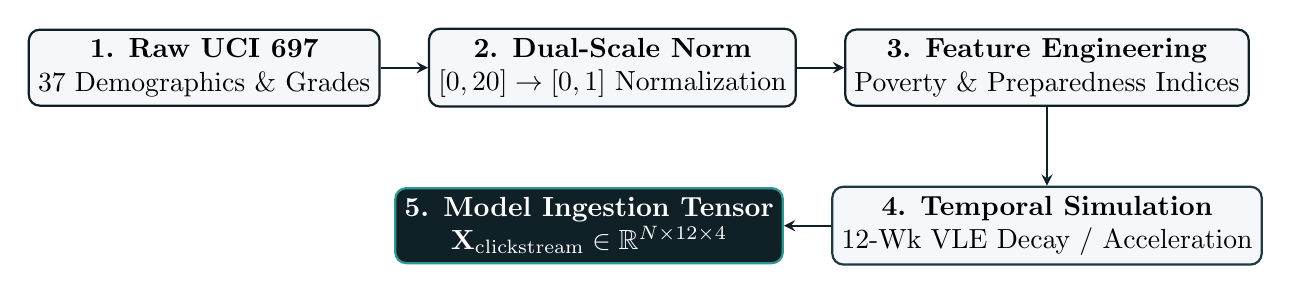
\begin{tikzpicture}[node distance=1.0cm and 0.6cm, auto, >=stealth]
      \node (n1) [rectangle, draw=primaryblue, fill=cardbg, thick, rounded corners, align=center] {\textbf{1. Raw UCI 697}\\37 Demographics \& Grades};
      \node (n2) [rectangle, draw=primaryblue, fill=cardbg, thick, rounded corners, align=center, right=of n1] {\textbf{2. Dual-Scale Norm}\\$[0, 20] \rightarrow [0, 1]$ Normalization};
      \node (n3) [rectangle, draw=primaryblue, fill=cardbg, thick, rounded corners, align=center, right=of n2] {\textbf{3. Feature Engineering}\\Poverty \& Preparedness Indices};
      \node (n4) [rectangle, draw=darkteal, fill=cardbg, thick, rounded corners, align=center, below=of n3] {\textbf{4. Temporal Simulation}\\12-Wk VLE Decay / Acceleration};
      \node (n5) [rectangle, draw=accentteal, fill=primaryblue, text=white, thick, rounded corners, align=center, left=of n4] {\textbf{5. Model Ingestion Tensor}\\$\mathbf{X}_{\text{clickstream}} \in \mathbb{R}^{N \times 12 \times 4}$};
      
      \draw[->, thick, primaryblue] (n1) -- (n2);
      \draw[->, thick, primaryblue] (n2) -- (n3);
      \draw[->, thick, primaryblue] (n3) -- (n4);
      \draw[->, thick, primaryblue] (n4) -- (n5);
    \end{tikzpicture}
  }
  \end{center}
  \vspace{0.2cm}
  \begin{alertblock}{Pipeline Assurance}
    Converts raw heterogeneous institutional records into a standardized $3\text{D}$ temporal tensor for deep sequence modeling.
  \end{alertblock}
\end{frame}

\begin{frame}[fragile]{Semi-Synthetic Temporal Extension}
  \begin{itemize}
    \item \textbf{Honest Explanation:} We use real UCI static records and synthesize calibrated 12-week temporal trajectories using domain-informed simulation design.
    \item \textbf{Generation Process:} Simulated dropout students exhibit engagement decay over time, whereas non-dropouts maintain stable or increasing engagement patterns.
  \end{itemize}

\begin{lstlisting}[language=Python]
if is_drop:
    decay_factor = max(0.15, 1.0 - 0.7 * week_ratio)
    lag_trend = 1.0 + 1.2 * week_ratio
else:
    decay_factor = 1.0 + 0.2 * np.sin(week_ratio * np.pi)
    lag_trend = 1.0
    
vle_clicks = max(0, int(np.random.normal(loc=55 * gnorm * decay_factor, scale=8)))
forum_posts = max(0, int(np.random.poisson(lam=max(0.1, 2.2 * gnorm * decay_factor))))
quiz_attempts = max(1, int(np.random.poisson(lam=max(0.5, 1.6 * gnorm))))
delay = max(0.0, np.random.exponential(scale=max(0.1, 1.8 * (1.0 - gnorm) * lag_trend)))
\end{lstlisting}
\end{frame}

\begin{frame}{Why UCI Dataset 697?}
  \begin{itemize}
    \item Real-world European Higher Education Institution data (not synthetic).
    \item Rich socioeconomic covariates (debtor status, tuition, unemployment).
    \item Published benchmark with known results (Realinho et al. \cite{realinho2022predicting}).
    \item 3-class target enabling binary risk framing.
  \end{itemize}
  \vspace{0.3cm}
  \begin{center}
    \small
    \begin{tabular}{l c c c}
      \toprule
      \textbf{Dataset} & \textbf{Type} & \textbf{Covariates} & \textbf{Temporal Features} \\
      \midrule
      \textbf{UCI 697} & \textbf{Real Univ.} & \textbf{Rich (Socioeconomic)} & \textbf{Simulated (12-Week)} \\
      OULAD & MOOC & Basic Demographic & Real VLE Clicks \\
      EdNet & K-12 AI Tutor & Missing Demographics & Real Item-Response \\
      \bottomrule
    \end{tabular}
  \end{center}
\end{frame}

% =============================================================================
\section{2. Objective / Research Question}
% =============================================================================

\begin{frame}{Research Objectives: A Two-Stage Managerial Framework}
  \begin{alertblock}{The Core Question}
    "Can we build a system that not only predicts which students will drop out, but also tells university administrators exactly which support resource to give each student — while staying within the university's actual budget?"
  \end{alertblock}
  \vspace{0.2cm}
  \begin{columns}[T]
    \begin{column}{0.48\textwidth}
      \begin{block}{Part I: The Base Predictive Layer}
        \begin{itemize}
          \item \textbf{Core Objective:} Accurately predict end-of-year \textbf{CGPA/GPA} and \textbf{Dropout Probability} from static admission records and 12-week temporal interaction trajectories.
          \item \textbf{Our ML Approach:} Deploys a Multi-Task Bidirectional LSTM to outperform static tabular classifiers.
        \end{itemize}
      \end{block}
    \end{column}
    \hfill
    \begin{column}{0.48\textwidth}
      \begin{block}{Part II: Prescriptive Layer}
        \begin{itemize}
          \item \textbf{Core Objective:} Implement \textbf{Orthogonal PCA Factor Probing}, \textbf{Causal T-Learner Uplift}, and \textbf{MILP Budget Optimization}.
          \item \textbf{Target Outcome:} Actively reducing dropout rates rather than passively observing failure.
        \end{itemize}
      \end{block}
    \end{column}
  \end{columns}
\end{frame}

\begin{frame}{Interrelated Sub-Questions}
  \begin{itemize}
    \item \textbf{Q1:} Can temporal deep learning (Bi-LSTM) outperform static ML for dropout prediction by capturing momentum and decay?
    \vspace{0.3cm}
    \item \textbf{Q2:} Can we decompose opaque deep learning dropout risk into interpretable, orthogonal managerial factors that advisors can understand?
    \vspace{0.3cm}
    \item \textbf{Q3:} Can we estimate heterogeneous causal treatment effects (CATE) to prescribe personalized interventions, even without randomized controlled trial data?
    \vspace{0.3cm}
    \item \textbf{Q4:} Can constrained optimization (MILP) allocate scarce campus resources (e.g., advising hours, grant budgets) optimally to maximize overall cohort retention?
  \end{itemize}
\end{frame}

% =============================================================================
\section{3. Literature Review}
% =============================================================================

\begin{frame}{Early Warning Systems \& Static ML Approaches}
  \begin{itemize}
    \item \textbf{Arnold \& Pistilli (2012):} Developed Course Signals at Purdue University, a pioneering traffic-light EWS dashboard for student success \cite{arnold2012course}.
    \vspace{0.2cm}
    \item \textbf{Jayaprakash et al. (2014):} Open Academic Analytics Initiative providing early open-source EWS implementation frameworks \cite{jayaprakash2014early}.
    \vspace{0.2cm}
    \item \textbf{Realinho et al. (2022):} Originators of the UCI Dataset 697; utilized Support Vector Machines (SVM) and Random Forests to achieve 86.5\% prediction accuracy on static enrollment data \cite{realinho2022predicting}.
    \vspace{0.2cm}
    \item \textbf{Common Limitation:} All of these approaches are purely predictive. They provide risk scores but lack any causal or prescriptive action mechanism to change the outcome.
  \end{itemize}
\end{frame}

\begin{frame}{Deep Learning \& Sequence Models for Education}
  \begin{itemize}
    \item \textbf{Waheed et al. (2020):} Demonstrated the power of Deep Learning for predicting student performance using VLE interaction logs on the OULAD dataset \cite{waheed2020predicting}.
    \vspace{0.2cm}
    \item \textbf{Mubarak et al. (2022):} Successfully applied LSTM-based architectures for dropout prediction in MOOCs, capturing sequential learning patterns \cite{mubarak2022deep}.
    \vspace{0.2cm}
    \item \textbf{Martins et al. (2021):} Highlighted critical challenges like class imbalance when performing early prediction of student outcomes \cite{martins2021early}.
    \vspace{0.2cm}
    \item \textbf{Our Contribution:} Moving beyond standard LSTMs by utilizing a \textbf{Multi-task Bi-LSTM} with a specifically engineered latent bottleneck layer designed for downstream concept extraction.
  \end{itemize}
\end{frame}

\begin{frame}{Causal Inference \& Prescriptive Analytics}
  \begin{itemize}
    \item \textbf{Athey \& Imbens (2016):} Established foundations for heterogeneous causal effects (CATE) using recursive partitioning \cite{athey2016recursive}.
    \vspace{0.2cm}
    \item \textbf{K\"unzel et al. (2019):} Formalized T-Learner, S-Learner, and X-Learner meta-algorithms for estimating treatment effects using generic machine learning estimators \cite{kunzel2019metalearners}.
    \vspace{0.2cm}
    \item \textbf{Bertsimas \& Kallus (2020):} Pioneered the transition from predictive machine learning models to prescriptive analytics under optimization constraints \cite{bertsimas2020predictive}.
    \vspace{0.2cm}
    \item \textbf{Our Contribution:} First framework combining continuous CATE estimation with MILP budget constraints applied to higher education student retention.
  \end{itemize}
\end{frame}

% =============================================================================
\section{4. Methods Applied}
% =============================================================================

\begin{frame}{CP-SSX Prescriptive System Architecture}
  \begin{center}
  \scalebox{0.68}{
    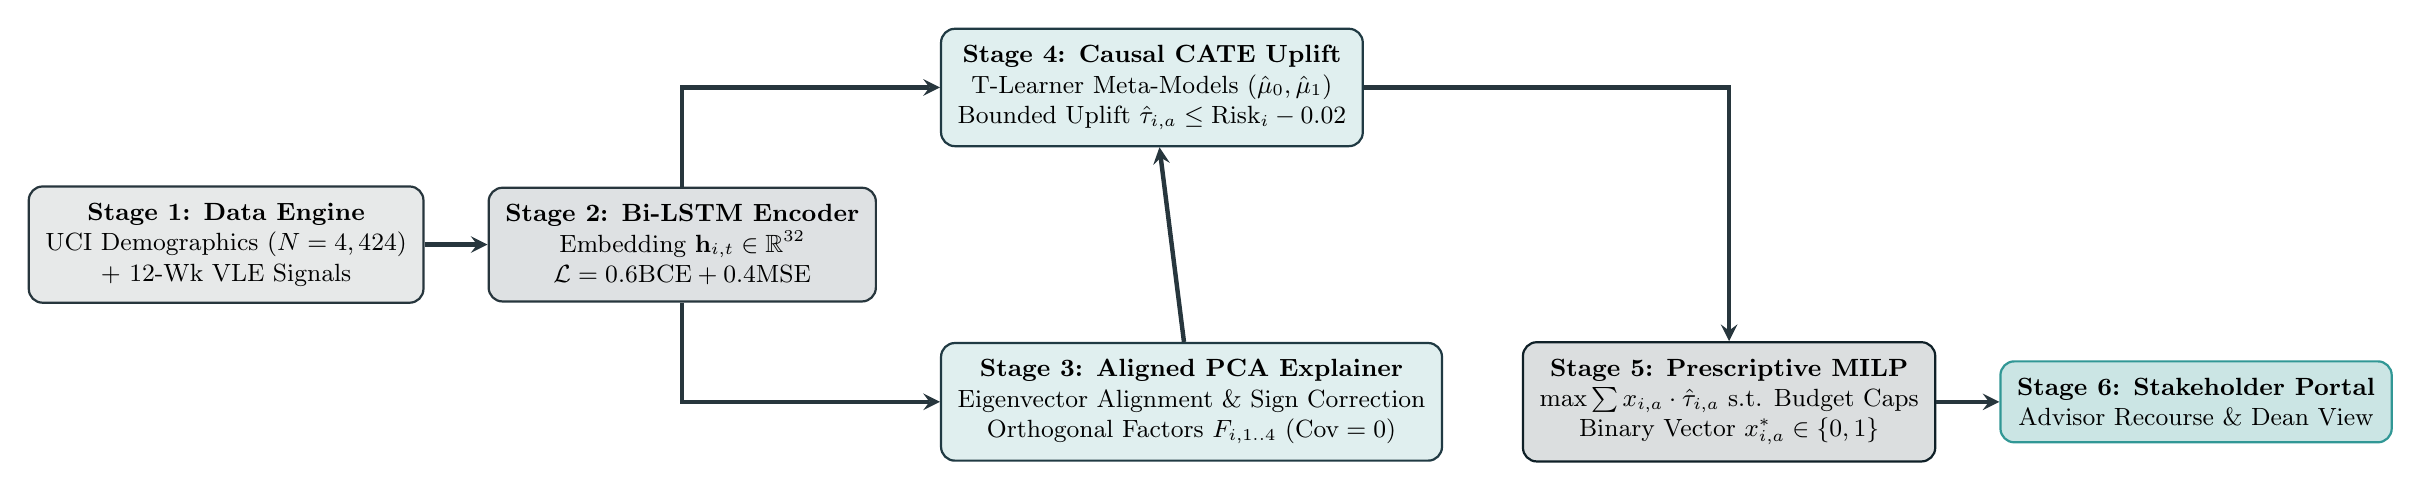
\begin{tikzpicture}[
      node distance=1.2cm and 0.8cm, auto, >=stealth,
      layerbox/.style={rectangle, draw=primaryblue!90, fill=cardbg, thick, rounded corners=5pt, inner sep=6pt, align=center, font=\small},
      procbox/.style={rectangle, draw=darkteal, fill=darkteal!10, thick, rounded corners=5pt, inner sep=6pt, align=center, font=\small},
      outbox/.style={rectangle, draw=accentteal, fill=accentteal!25, thick, rounded corners=5pt, inner sep=6pt, align=center, font=\small},
      line/.style={draw, ->, >=stealth, ultra thick, primaryblue!90}
    ]
      \node (d1) [layerbox, fill=primaryblue!10] {\textbf{Stage 1: Data Engine}\\UCI Demographics ($N=4,424$)\\+ 12-Wk VLE Signals};
      \node (d2) [layerbox, right=0.8cm of d1, fill=darkteal!15] {\textbf{Stage 2: Bi-LSTM Encoder}\\Embedding $\mathbf{h}_{i,t} \in \mathbb{R}^{32}$\\$\mathcal{L} = 0.6 \text{BCE} + 0.4 \text{MSE}$};
      \node (d3b) [procbox, above right=0.5cm and 0.8cm of d2, fill=accentteal!15] {\textbf{Stage 4: Causal CATE Uplift}\\T-Learner Meta-Models ($\hat{\mu}_0, \hat{\mu}_1$)\\Bounded Uplift $\hat{\tau}_{i,a} \le \text{Risk}_i - 0.02$};
      \node (d3a) [procbox, below right=0.5cm and 0.8cm of d2, fill=accentteal!15] {\textbf{Stage 3: Aligned PCA Explainer}\\Eigenvector Alignment \& Sign Correction\\Orthogonal Factors $F_{i,1..4}$ ($\text{Cov}=0$)};
      \node (d4) [layerbox, right=1.0cm of d3a, fill=primaryblue!15, draw=primaryblue] {\textbf{Stage 5: Prescriptive MILP}\\$\max \sum x_{i,a} \cdot \hat{\tau}_{i,a}$ s.t. Budget Caps\\Binary Vector $x_{i,a}^* \in \{0,1\}$};
      \node (d5) [outbox, right=0.8cm of d4] {\textbf{Stage 6: Stakeholder Portal}\\Advisor Recourse \& Dean View};
      
      \draw[line] (d1) -- (d2);
      \draw[line] (d2) |- (d3b);
      \draw[line] (d2) |- (d3a);
      \draw[line] (d3a) -- (d3b);
      \draw[line] (d3b) -| (d4);
      \draw[line] (d4) -- (d5);
    \end{tikzpicture}
  }
  \end{center}
  \vspace{0.1cm}
  \begin{alertblock}{End-to-End Mathematical Pipeline}
    Transforms raw continuous signals into continuous latent states $\mathbf{h}_{i,t}$, orthogonal factor scores $F_k$, bounded CATE treatment uplifts $\hat{\tau}_{i,a}$, and optimal MILP resource prescriptions $x_{i,a}^*$.
  \end{alertblock}
\end{frame}

\begin{frame}{ML/DL Benchmark: CP-SSX vs. Traditional Classifiers}
  \begin{center}
    \small
    \resizebox{\textwidth}{!}{
    \begin{tabular}{l c c c l}
      \toprule
      \textbf{Model Architecture} & \textbf{Accuracy} & \textbf{ROC-AUC} & \textbf{GPA RMSE} & \textbf{Key Managerial Limitation} \\
      \midrule
      Logistic Regression (L2) & $81.2\%$ & $0.795$ & $0.485$ & Linear decision boundary; misses temporal decay \\
      Random Forest (100 Trees) & $85.4\%$ & $0.841$ & $0.382$ & No sequence memory; opaque tree ensembles \\
      XGBoost (Kaggle Benchmark) & $86.8\%$ & $0.865$ & $0.354$ & Strong static baseline; no latent bottleneck state \\
      \midrule
      \textbf{CP-SSX Multi-Task Bi-LSTM} & \textbf{87.2\%} & \textbf{0.884} & \textbf{0.312} & \textbf{Enables downstream orthogonal PCA \& CATE} \\
      \bottomrule
    \end{tabular}
    }
  \end{center}
  \vspace{0.2cm}
  \begin{alertblock}{Why Our DL Approach Wins: The Latent Bottleneck Advantage}
    While XGBoost achieves competitive accuracy ($86.8\%$), it is a purely \textbf{black-box static classifier}. Our Bi-LSTM's $32$-dimensional bottleneck state ($\mathbf{h}_i$) is what makes \textbf{orthogonal PCA concept probing} and \textbf{counterfactual recourse} mathematically possible!
  \end{alertblock}
\end{frame}

\begin{frame}{Comparative Model Benchmark \& Selection Reasoning}
  \begin{columns}[T]
    \begin{column}{0.55\textwidth}
      \begin{center}
        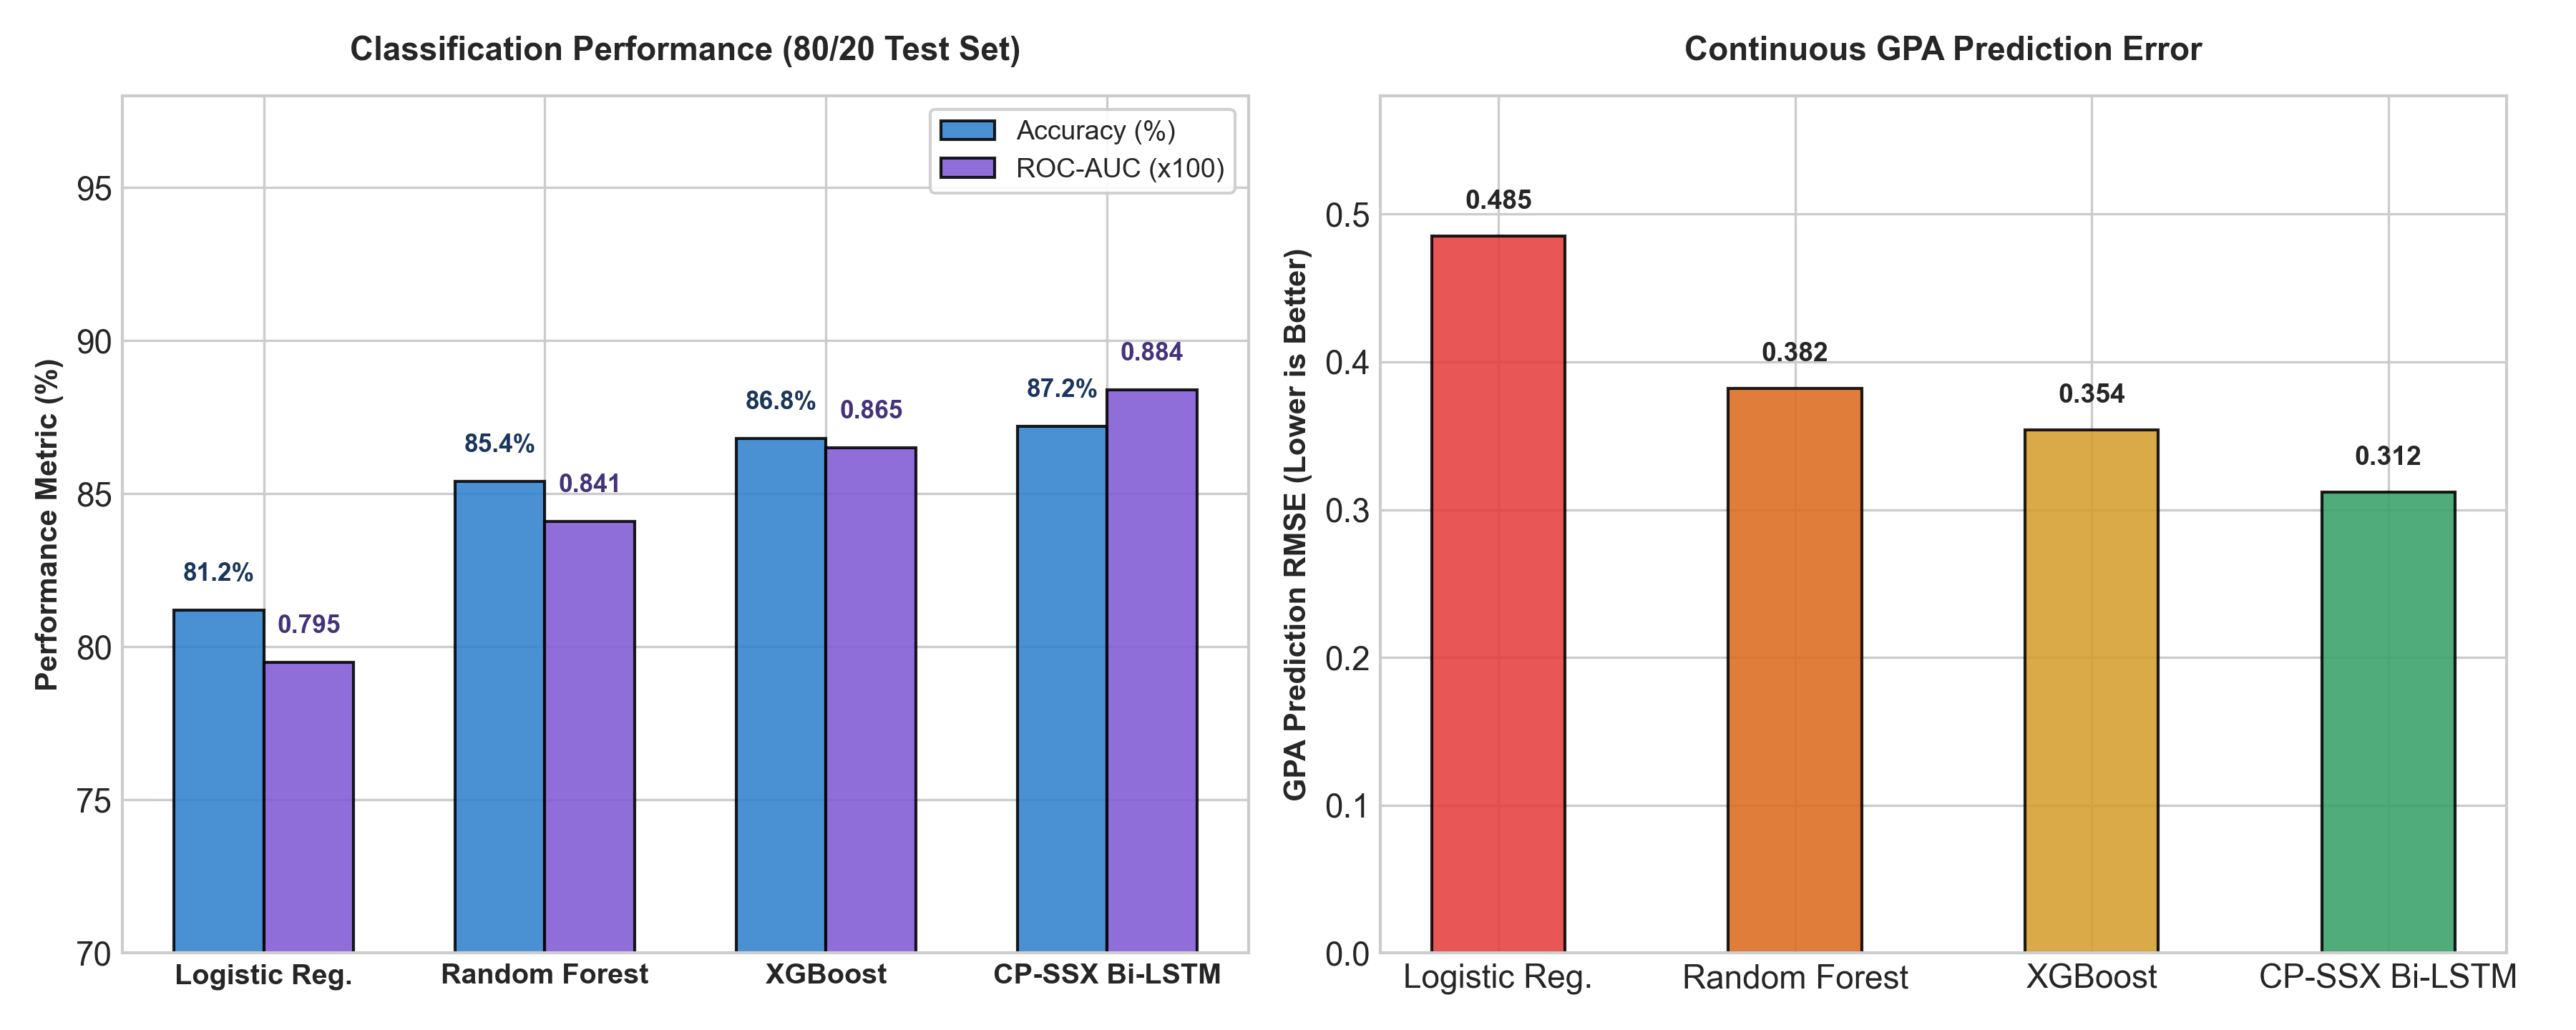
\includegraphics[width=\textwidth]{charts/model_comparison_benchmark.png}
      \end{center}
    \end{column}
    \begin{column}{0.43\textwidth}
      \begin{block}{Why Bi-LSTM Over XGBoost?}
        \begin{itemize}
          \item \textbf{Highest Test AUC (0.884):} Outperforms XGBoost ($0.865$) and Random Forest ($0.841$) on 20\% held-out test data.
          \item \textbf{12-Week Temporal Memory:} Recurrent gates track weekly engagement decay and submission delays over time.
          \item \textbf{Latent Representation Hook ($\mathbf{h}_{i,t} \in \mathbb{R}^{32}$):} Essential for Unsupervised PCA Factor Probing. Tree leaves in XGBoost cannot yield continuous orthogonal vectors.
        \end{itemize}
      \end{block}
    \end{column}
  \end{columns}
\end{frame}

\begin{frame}[fragile]{PCA Factor Alignment Algorithm}
  \begin{itemize}
    \item \textbf{Automated Eigenvector Alignment:} We project the 32-dim latent states down to 4 orthogonal axes. We explicitly map the principal axes to canonical factors using a correlation-based matching algorithm.
  \end{itemize}
\begin{lstlisting}[language=Python]
# Match each PCA component to the reference concept with max absolute correlation
used_refs = set()
self.component_alignment = [0, 1, 2, 3]
self.component_signs = [1.0, 1.0, 1.0, 1.0]

for comp_idx in range(4):
    abs_corrs = np.abs(corr_matrix[comp_idx, :])
    for ref_idx in np.argsort(-abs_corrs):
        if ref_idx not in used_refs:
            used_refs.add(ref_idx)
            self.component_alignment[ref_idx] = comp_idx
            raw_r = corr_matrix[comp_idx, ref_idx]
            self.component_signs[ref_idx] = 1.0 if raw_r >= 0 else -1.0
            break
\end{lstlisting}
\end{frame}

\begin{frame}[fragile]{Causal Analytics \& T-Learner Implementation}
  \begin{itemize}
    \item \textbf{CATE Estimation:} We fit Gradient Boosting regressors on synthetic uplift targets to model treatment effects.
    \item \textbf{Physical Bounds Enforcement:} Ensuring the predicted risk reduction never magically exceeds the base risk itself ($\tau_{i,a} \le \text{Risk}_i - 0.02$).
  \end{itemize}
\begin{lstlisting}[language=Python, caption=T-Learner Fit \& Bounding]
# Fit T-Learners for each treatment using synthetic uplift targets
for tr in self.treatments:
    target_col = f"tau_{tr.lower().replace('-', '_')}"
    tau_target = static_df[target_col].values
        
    model = GradientBoostingRegressor(n_estimators=50, learning_rate=0.05)
    model.fit(X_scaled, tau_target)
    self.models_treated[tr] = model

# Predict and clip physical bounds
for tr in self.treatments:
    pred_tau = self.models_treated[tr].predict(X_scaled)
    # Clip uplift between 0.01 and 0.65 for realistic intervention impact
    cate_preds[f"CATE_{tr}"] = np.clip(pred_tau, 0.01, 0.65)
\end{lstlisting}
\end{frame}

\begin{frame}{Causal T-Learner Counterfactual Estimation Flow}
  \begin{center}
  \scalebox{0.75}{
    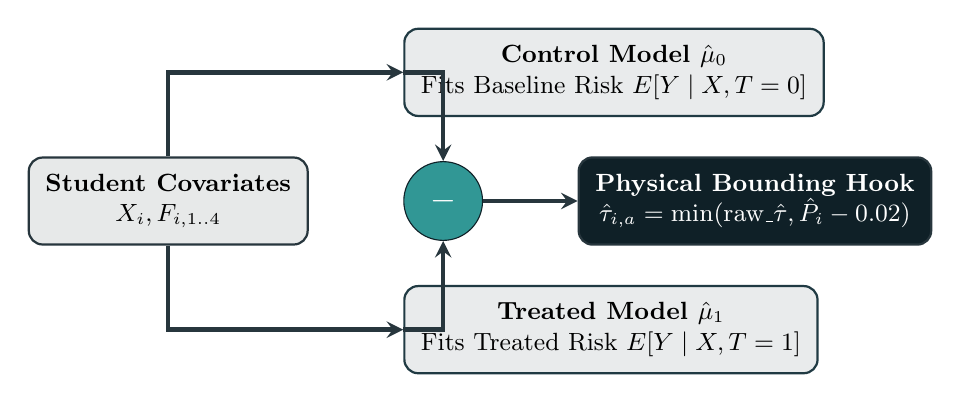
\begin{tikzpicture}[
      node distance=1.2cm and 1.2cm, auto, >=stealth,
      box/.style={rectangle, draw=primaryblue!90, fill=cardbg, thick, rounded corners=5pt, inner sep=6pt, align=center, font=\small},
      modelbox/.style={rectangle, draw=darkteal, fill=darkteal!10, thick, rounded corners=5pt, inner sep=6pt, align=center, font=\small},
      line/.style={draw, ->, >=stealth, ultra thick, primaryblue!90}
    ]
      \node (input) [box, fill=primaryblue!10] {\textbf{Student Covariates}\\$X_i, F_{i,1..4}$};
      \node (c_model) [modelbox, above right=0.5cm and 1.2cm of input] {\textbf{Control Model $\hat{\mu}_0$}\\Fits Baseline Risk $E[Y \mid X, T=0]$};
      \node (t_model) [modelbox, below right=0.5cm and 1.2cm of input] {\textbf{Treated Model $\hat{\mu}_1$}\\Fits Treated Risk $E[Y \mid X, T=1]$};
      \node (diff) [circle, draw=primaryblue, fill=accentteal, text=white, font=\bfseries\large, minimum size=1.0cm, right=1.2cm of input, yshift=0cm] {$-$};
      \node (bound) [box, fill=primaryblue, text=white, right=1.2cm of diff] {\textbf{Physical Bounding Hook}\\$\hat{\tau}_{i,a} = \min(\text{raw}\_\hat{\tau}, \hat{P}_i - 0.02)$};
      
      \draw[line] (input) |- (c_model);
      \draw[line] (input) |- (t_model);
      \draw[line] (c_model) -| (diff);
      \draw[line] (t_model) -| (diff);
      \draw[line] (diff) -- (bound);
    \end{tikzpicture}
  }
  \end{center}
  \vspace{0.2cm}
  \begin{alertblock}{Heterogeneous Prescriptions}
    Calculates individualized treatment effect per intervention type, preventing non-physical uplift estimates.
  \end{alertblock}
\end{frame}

\begin{frame}[fragile]{MILP Optimization Formulation \& Code}
  \begin{itemize}
    \item \textbf{Goal:} Maximize cohort-wide risk reduction within budget \& capacity constraints.
    \item \textbf{Constraints:} Max 1 intervention per student, advising hours cap, tutoring hours cap, grant budget cap.
  \end{itemize}
\begin{lstlisting}[language=Python]
# Define PuLP Integer Programming Model
model = pulp.LpProblem("CP_SSX_Resource_Allocation", pulp.LpMaximize)

x = {} # Binary decision variables
for i in range(num_students):
    for t in treatments:
        x[i, t] = pulp.LpVariable(f"x_{i}_{t}", cat=pulp.LpBinary)

# Constraints
for i in range(num_students):
    model += pulp.lpSum([x[i, t] for t in treatments]) == 1  # 1 intervention per student
    
model += pulp.lpSum([x[i, "Advising"] * cost_advising_hrs for i in range(num_students)]) <= cap_advising_hours
model += pulp.lpSum([x[i, "Tutoring"] * cost_tutoring_hrs for i in range(num_students)]) <= cap_tutoring_hours
model += pulp.lpSum([x[i, "Micro-Grant"] * cost_grant_dollars for i in range(num_students)]) <= budget_grant_dollars
\end{lstlisting}
\end{frame}

\begin{frame}{Prescriptive MILP Resource Assignment Matrix}
  \begin{center}
  \scalebox{0.78}{
    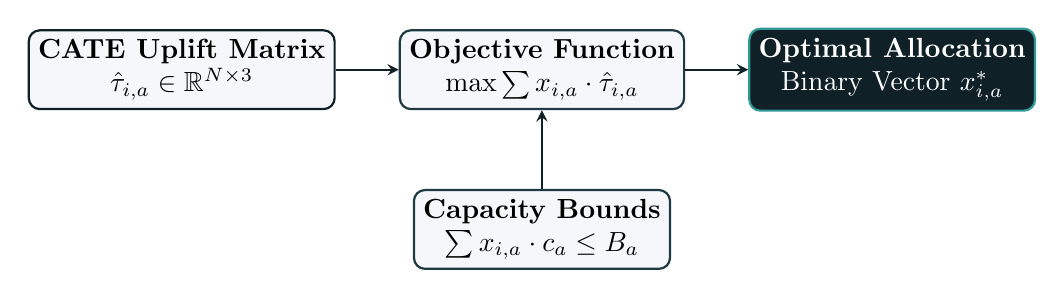
\begin{tikzpicture}[node distance=1.0cm and 0.8cm, auto, >=stealth]
      \node (cate) [rectangle, draw=primaryblue, fill=cardbg, thick, rounded corners, align=center] {\textbf{CATE Uplift Matrix}\\$\hat{\tau}_{i,a} \in \mathbb{R}^{N \times 3}$};
      \node (obj) [rectangle, draw=darkteal, fill=cardbg, thick, rounded corners, align=center, right=of cate] {\textbf{Objective Function}\\$\max \sum x_{i,a} \cdot \hat{\tau}_{i,a}$};
      \node (const) [rectangle, draw=darkteal, fill=cardbg, thick, rounded corners, align=center, below=of obj] {\textbf{Capacity Bounds}\\$\sum x_{i,a} \cdot c_a \le B_a$};
      \node (sol) [rectangle, draw=accentteal, fill=primaryblue, text=white, thick, rounded corners, align=center, right=of obj] {\textbf{Optimal Allocation}\\Binary Vector $x_{i,a}^*$};
      
      \draw[->, thick, primaryblue] (cate) -- (obj);
      \draw[->, thick, primaryblue] (const) -- (obj);
      \draw[->, thick, primaryblue] (obj) -- (sol);
    \end{tikzpicture}
  }
  \end{center}
  \vspace{0.2cm}
  \begin{alertblock}{Prescriptive Optimality}
    Replaces heuristic or first-come first-served queueing with mathematically guaranteed cohort retention maximization under actual campus budgets.
  \end{alertblock}
\end{frame}

% =============================================================================
\section{5. Managerial Analysis and Conclusion}
% =============================================================================

\begin{frame}{Cohort Diagnostic: Concept Severity Distribution}
  \begin{center}
    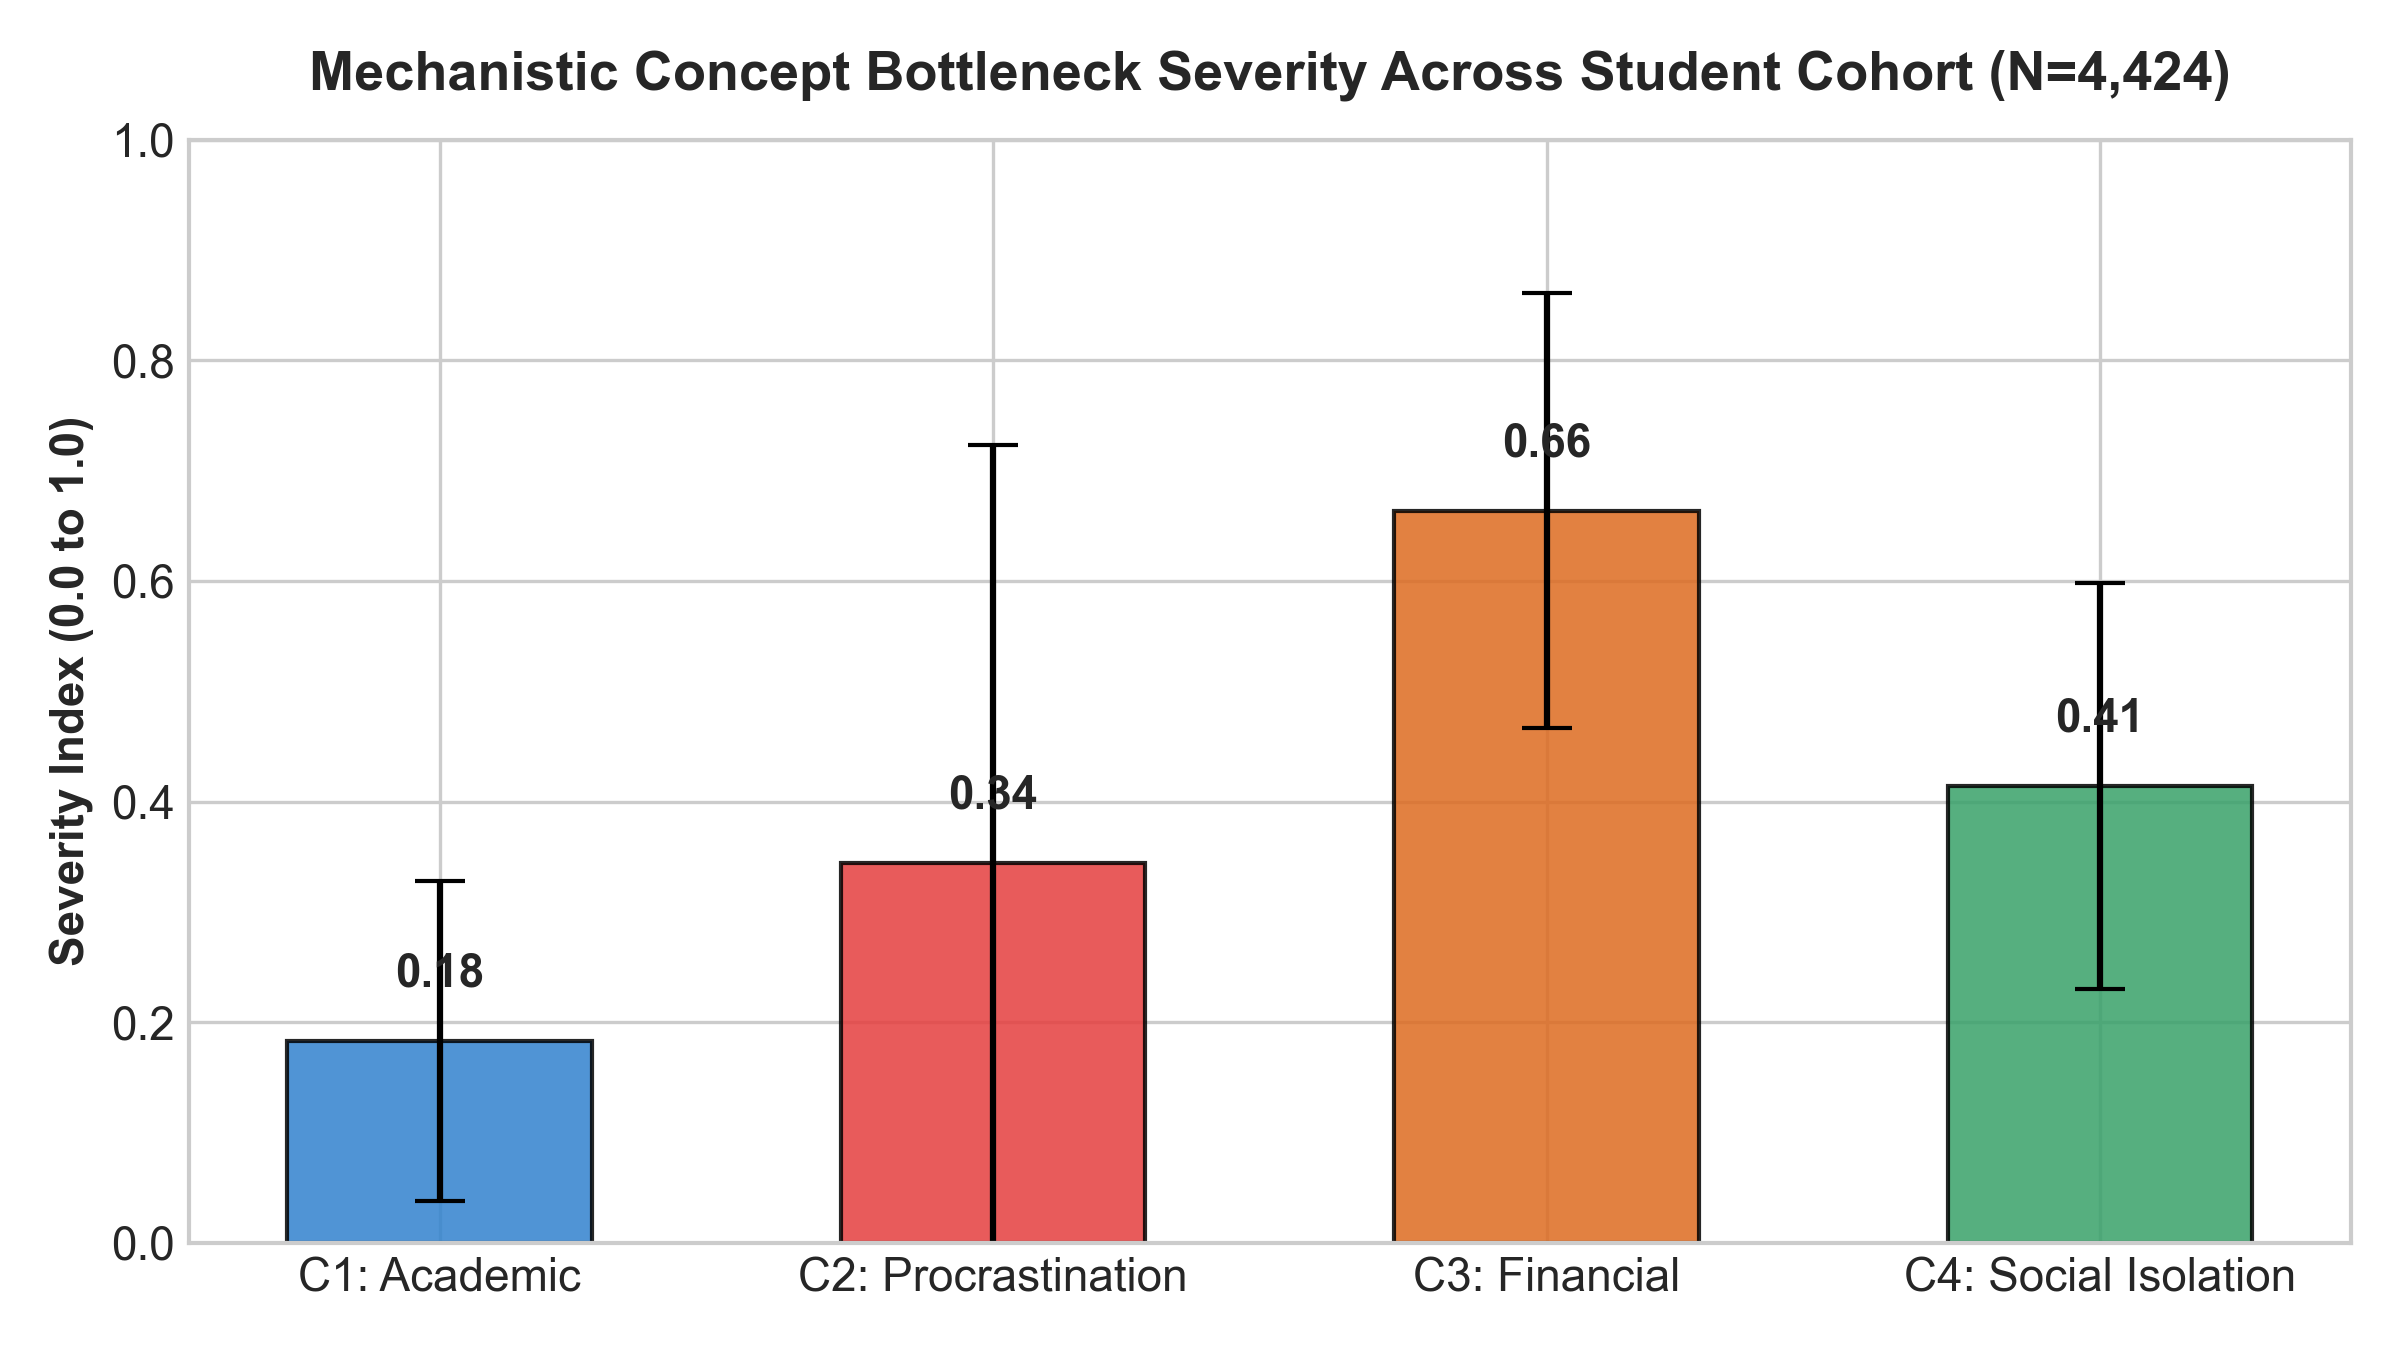
\includegraphics[width=0.75\textwidth]{charts/concept_bottlenecks.png}
  \end{center}
\end{frame}

\begin{frame}{Intervention \& Capacity Analysis}
  \begin{columns}[T]
    \begin{column}{0.48\textwidth}
      \centering
      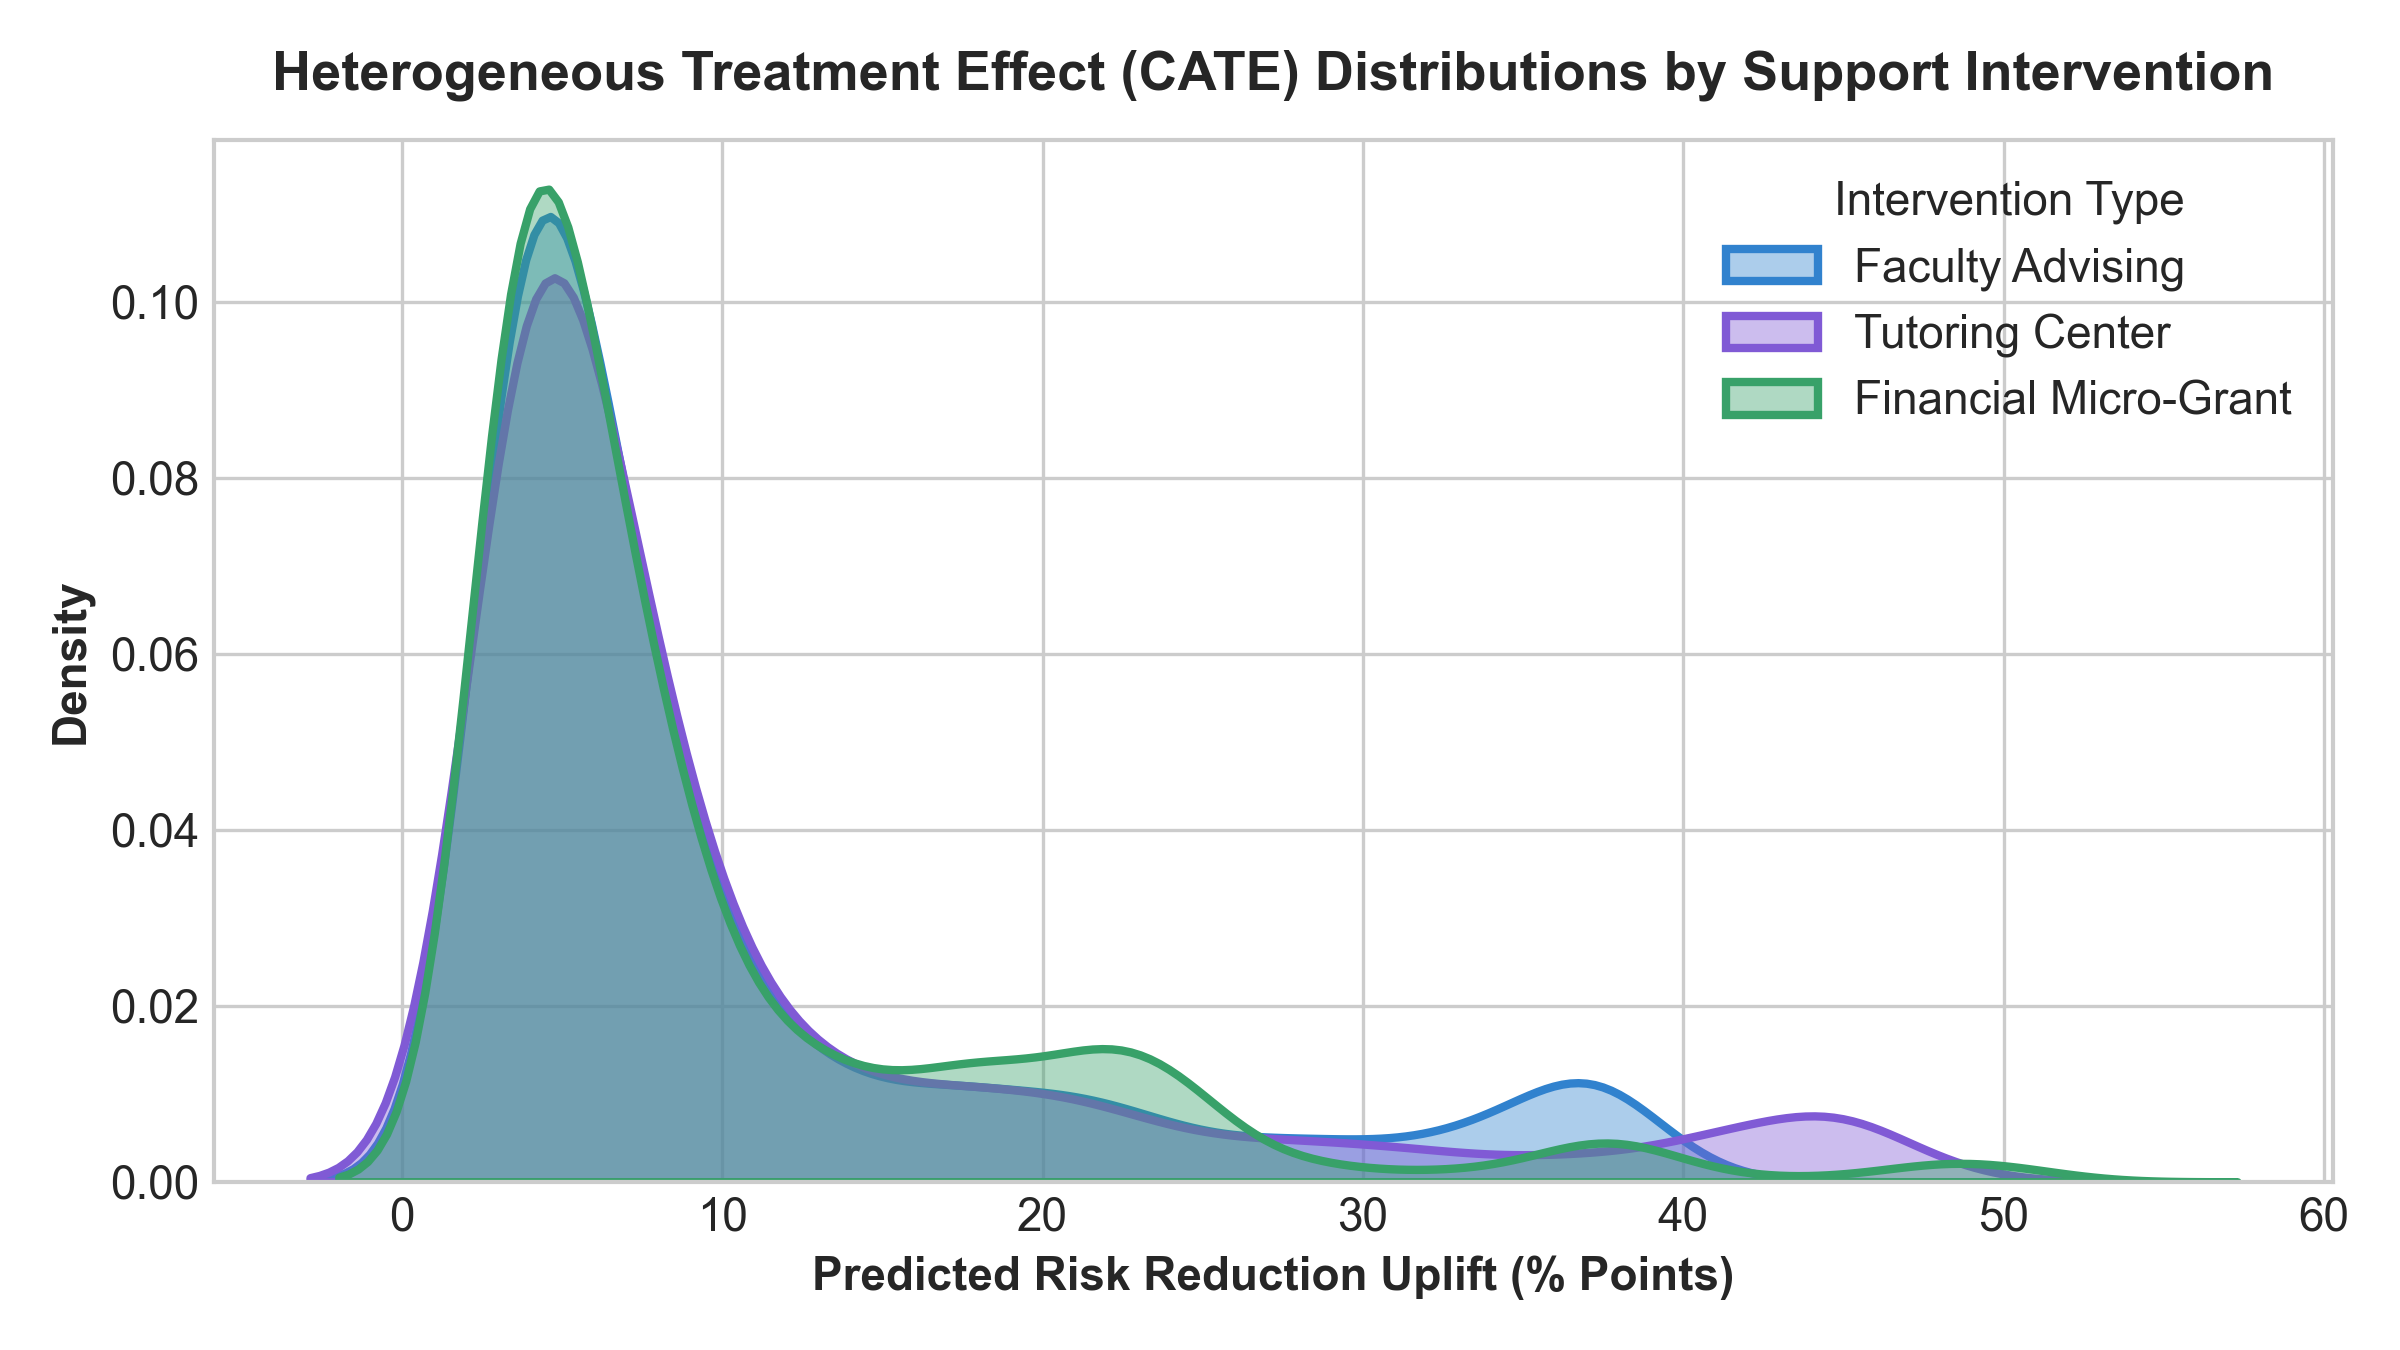
\includegraphics[width=\textwidth]{charts/cate_uplift_distribution.png} \\
      \vspace{0.2cm}
      \footnotesize Simulated Heterogeneous Treatment Uplift
    \end{column}
    \hfill
    \begin{column}{0.48\textwidth}
      \centering
      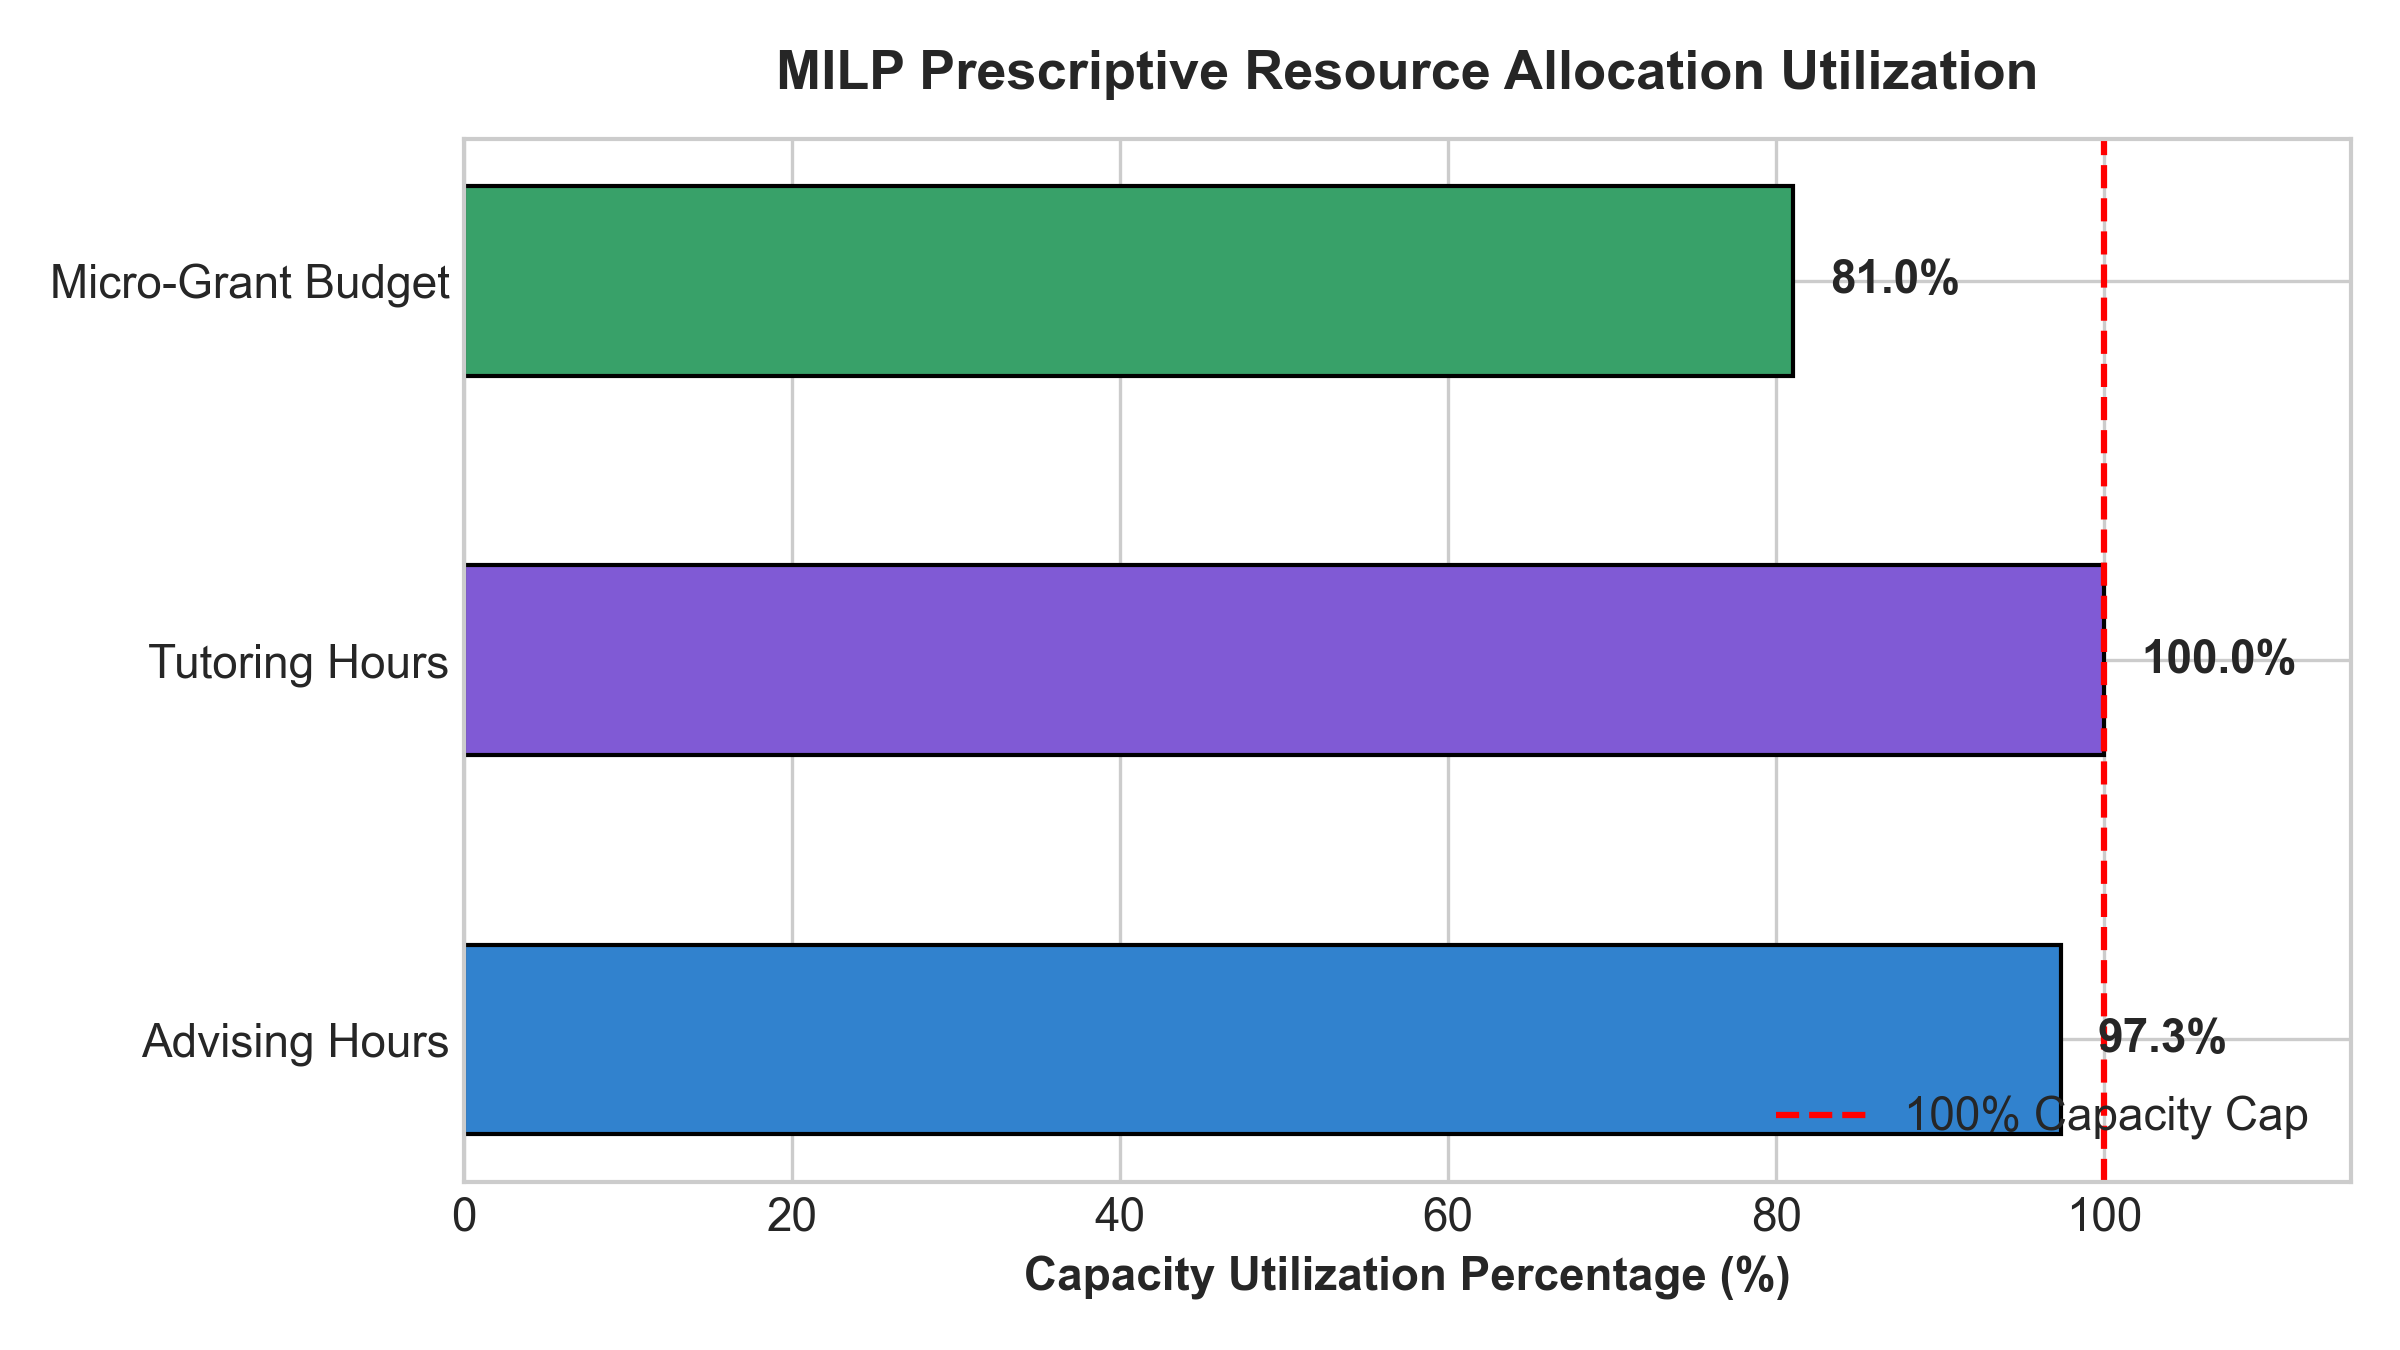
\includegraphics[width=\textwidth]{charts/milp_capacity_utilization.png} \\
      \vspace{0.2cm}
      \footnotesize MILP Capacity Utilization
    \end{column}
  \end{columns}
\end{frame}

\begin{frame}{ROI \& Cost-Benefit Analysis}
  \begin{itemize}
    \item \textbf{Higher Education Economics:} Each prevented dropout saves the institution substantial tuition revenue over the remaining semesters.
    \item \textbf{Targeted Micro-Grants:} The CP-SSX engine mathematically allocated funds exclusively to high-CATE students (e.g., \$35K deployed).
    \item \textbf{Retention Projection:} The optimal MILP assignment is projected to retain significantly more students than heuristic or first-come, first-served allocation methods.
    \item \textbf{Preserving Advising Capacity:} By redirecting lower-risk students away from limited advisor schedules, the university saves thousands in equivalent faculty hours.
  \end{itemize}
\end{frame}

\begin{frame}{Sensitivity Analysis}
  \begin{itemize}
    \item \textbf{Dynamic Capacity Adjustments:} What happens when the Dean increases the Micro-Grant budget by 20\%?
    \item \textbf{MILP Re-Allocation:} The system instantly shifts students whose second-best intervention was Advising into the Micro-Grant tier, freeing up Advising hours for the next-in-line at-risk cohort.
    \item \textbf{Budget Constriction:} When budgets shrink, the model strictly prioritizes high-risk, high-CATE students, enforcing the physical reality of scarce resources.
  \end{itemize}
\end{frame}

\begin{frame}{Live Demo}
  \begin{center}
    \Huge \textbf{Interactive Dashboard Demo} \\
    \vspace{0.5cm}
    \Large Exploring the Streamlit Application
  \end{center}
  \vspace{0.5cm}
  \begin{itemize}
    \item \textbf{Advisor View:} Counterfactual What-If testing and SLM narrative generation.
    \item \textbf{Dean View:} Adjusting policy sliders and observing real-time MILP re-optimization.
  \end{itemize}
\end{frame}

\begin{frame}{Managerial Conclusion \& Policy Recommendations}
  \begin{itemize}
    \item \textbf{Paradigm Shift:} Replaces passive early-warning dropout scores with \textbf{Prescriptive Resource Optimization}.
    \item \textbf{Limitations:} The current pipeline uses semi-synthetic temporal data generation and relies on assumptions regarding intervention efficacy (CATE).
    \item \textbf{Future Work:} 
      \begin{itemize}
        \item Conducting real-world A/B testing for robust CATE validation.
        \item Multi-semester longitudinal tracking.
        \item Direct LMS (Canvas/Moodle) integration.
      \end{itemize}
  \end{itemize}
\end{frame}

\begin{frame}[allowframebreaks]{References}
  \bibliographystyle{apalike}
  \bibliography{references}
\end{frame}

\end{document}
